\section{Progressive Networks}

Continual learning is a long-standing goal of machine learning, where agents
not only learn (and remember) a series of tasks experienced in sequence, but also have
the ability to transfer knowledge from previous tasks to improve convergence speed \cite{AAAIMag11-Taylor}.
\textit{Progressive networks} integrate these desiderata directly into the
model architecture: catastrophic forgetting is prevented by instantiating a new
neural network (a \textit{column}) for each task being solved, while transfer is
enabled via lateral connections to features of previously learned columns. The
scalability of this approach is addressed at the end of this section.

A progressive network starts with a single column: a deep neural network having
$L$ layers with hidden activations $h_i^{(1)} \in \mathbb{R}^{n_i}$,
with $n_i$ the number of units at layer $i \le L$, and parameters
$\Theta^{(1)}$ trained to convergence.  When switching to a second task, the
parameters $\Theta^{(1)}$ are ``frozen'' and a new
column with parameters $\Theta^{(2)}$ is instantiated (with random
initialization), where layer $h_i^{(2)}$ receives input from both
$h_{i-1}^{(2)}$ and $h_{i-1}^{(1)}$ via lateral connections. This
generalizes to $K$ tasks as follows:
\footnote{Progressive networks can also be generalized in a straightforward
manner to have arbitrary network width per column/layer, to accommodate varying
degrees of task difficulty, or to compile lateral connections from multiple,
independent networks in an ensemble setting. Biases are omitted for clarity.}:
\begin{align}
  \label{eq:prognet}
  h_i^{(k)} = f\left( W_i^{(k)} h_{i-1}^{(k)} + \sum_{j<k} U_{i}^{(k:j)} h_{i-1}^{(j)} \right),
\end{align}
where $W_i^{(k)} \in \mathbb{R}^{n_{i} \times n_{i-1}}$ is the weight matrix of layer
$i$ of column $k$, $U_{i}^{(k:j)} \in \mathbb{R}^{n_i \times n_j}$ are the
lateral connections from layer $i-1$ of column $j$, to layer $i$ of column $k$
and $h_0$ is the network input.
$f$ is an element-wise non-linearity: we use $f(x)=\max(0, x)$ for all
intermediate layers.
A progressive network with $K=3$ is shown in Figure~\ref{fig:progressiveNet}.

\begin{figure}[h]
  \centering
    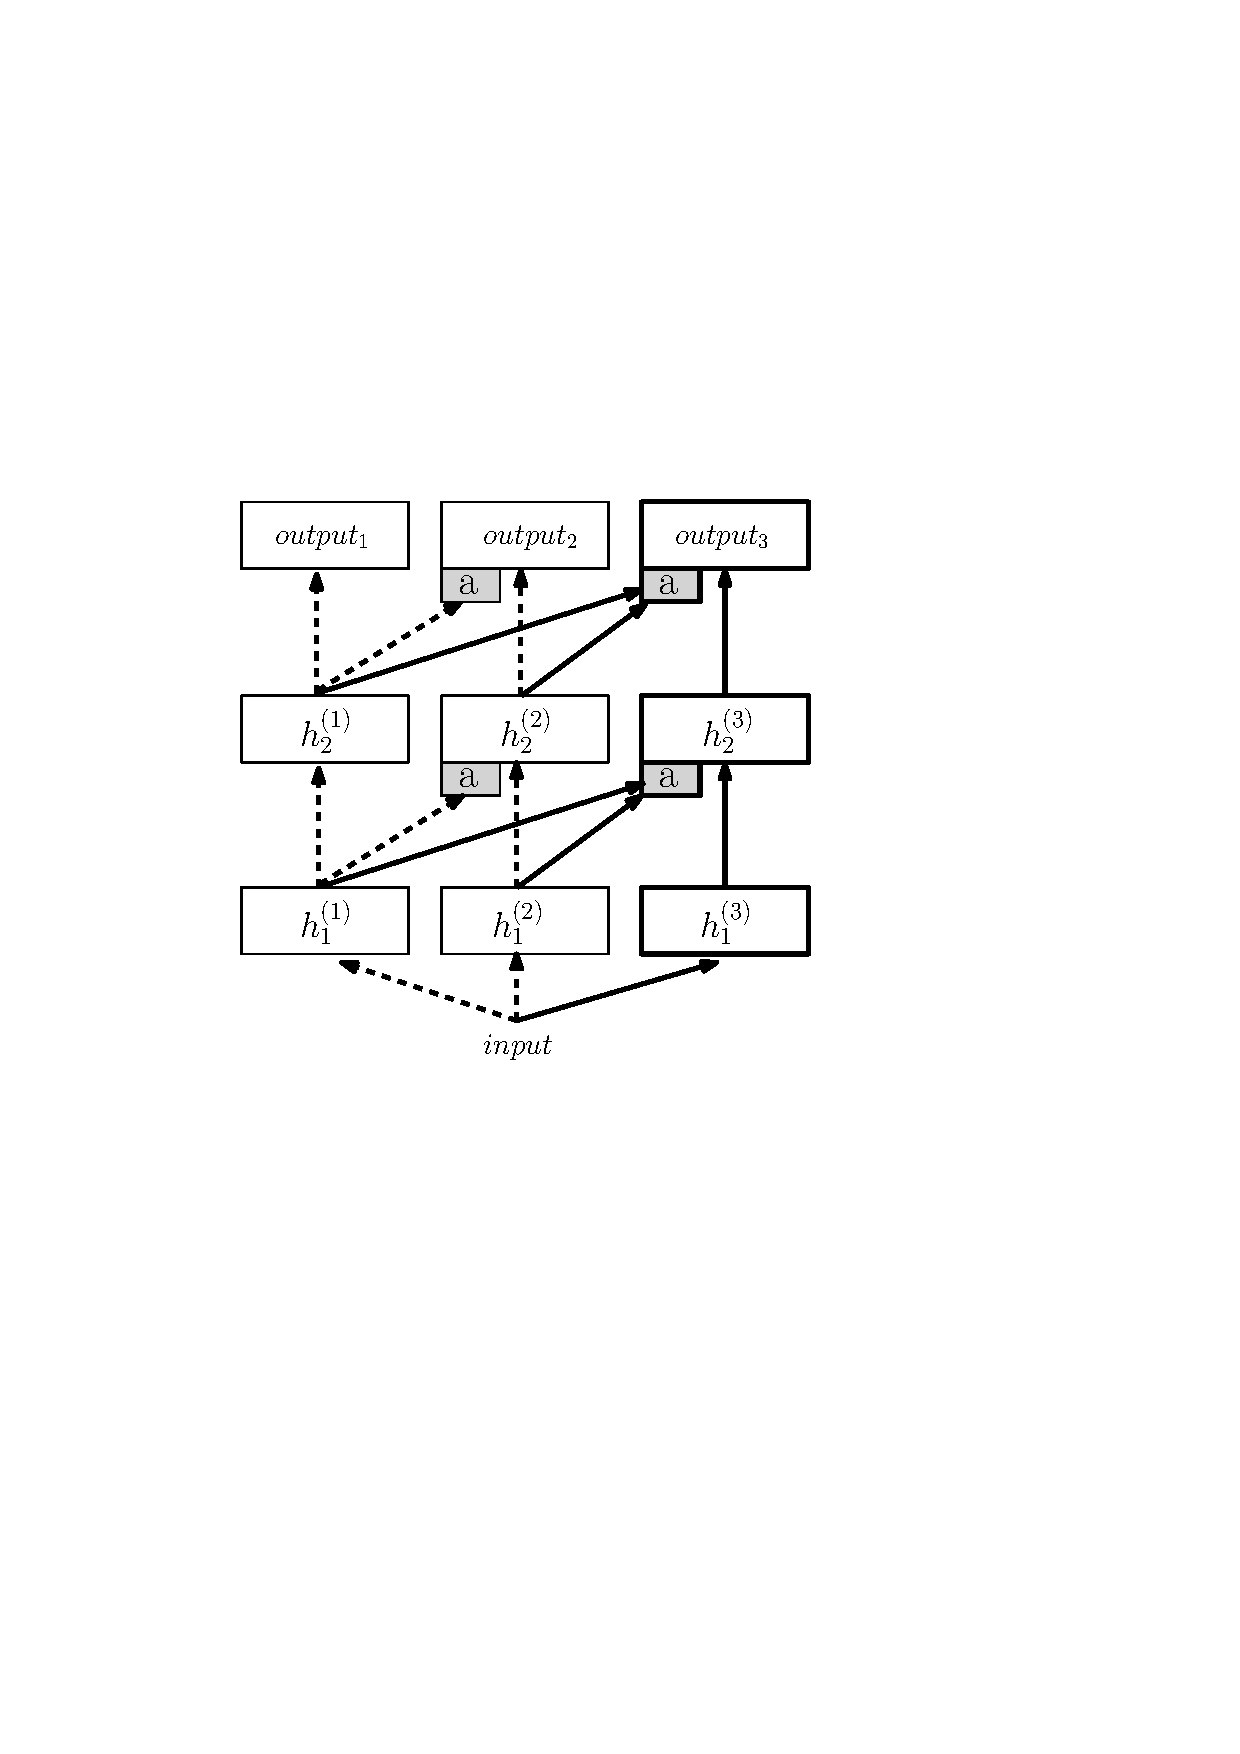
\includegraphics[width=.25\textwidth]{figures/progressiveNetDepiction2}
    \caption{Depiction of a three column progressive network. The first two
columns on the left (dashed arrows) were trained on task 1 and 2 respectively.
The grey box labelled $a$ represent the adapter layers (see text).
A third column is added for the final task having access to all previously learned
features.
    }
    \label{fig:progressiveNet}
\end{figure}

These modelling decisions are informed by our desire to:
(1) solve $K$ independent tasks at the end of training;
(2) accelerate learning via transfer when possible; and
(3) avoid catastrophic forgetting.

In the standard pretrain-and-finetune paradigm, there is often an implicit
assumption of ``overlap'' between the tasks. Finetuning is efficient in this
setting, as parameters need only be adjusted slightly to
the target domain, and often only the top layer is retrained \cite{yosinski-nips2014}. In contrast, we make no assumptions about the
relationship between tasks, which may in practice be orthogonal or even
adversarial. While the finetuning stage could potentially unlearn these
features, this may prove difficult. Progressive networks side-step
this issue by allocating a new column for each new task, whose weights are
initialized randomly. Compared to the task-relevant initialization of pretraining,
columns in progressive networks are free to reuse, modify or ignore previously
learned features via the lateral connections.
As the lateral connections $U_{i}^{(k:j)}$ are only from column $k$ to columns
$j < k$, previous columns are not affected by the newly learned features in the
forward pass.  Because also the parameters $\{ \Theta^{(j)}; j<k\}$
are kept frozen (i.e. are constants for the optimizer) when training $\Theta^{(k)}$,
there is no interference between
tasks and hence no catastrophic forgetting.

\paragraph{Application to Reinforcement Learning.} Although progressive
networks are widely applicable, this paper focuses on their application to
deep reinforcement learning. In this case, each column is trained to solve a
particular Markov Decision Process (MDP): the $k$-th column thus defines a policy
$\pi^{(k)}(a\mid s)$ taking as input a state $s$ given by the environment,
and generating probabilities over actions $\pi^{(k)}(a\mid s) := h_L^{(k)}(s)$.
At each time-step, an action is sampled from this distribution and taken in the
environment, yielding the subsequent state. This policy implicitly defines a
stationary distribution $\rho_{\pi^{(k)}}(s,a)$ over states and actions.

\paragraph{Adapters.}
In practice, we augment the progressive network layer of Equation~\ref{eq:prognet} with
non-linear lateral connections which we call \textit{adapters}. They serve
both to improve initial conditioning and perform dimensionality reduction.
Defining the vector of anterior features
$h_{i-1}^{(<k)} = [h_{i-1}^{(1)} \cdots h_{i-1}^{(j)} \cdots h_{i-1}^{(k-1)}]$
of dimensionality $n_{i-1}^{(<k)}$, in the case of dense layers,
we replace the linear lateral connection with a single hidden layer MLP.
Before feeding the lateral activations into the MLP, we multiply them by a learned scalar,
initialized by a random small value.
Its role is to adjust for the different scales of the different inputs.
The hidden layer of the non-linear adapter is a projection onto an $n_{i}$ dimensional
subspace.  As the
index $k$ grows, this ensures that the number of parameters stemming from the
lateral connections is in the same order as $\left|\Theta^{(1)} \right|$. Omitting bias
terms, we get:
\begin{align}
  \label{eq:prognet}
  h_i^{(k)} = \sigma \left( W_i^{(k)} h_{i-1}^{(k)} + U_{i}^{(k:j)} \sigma(V_{i}^{(k:j)} \alpha_{i-1}^{(<k)} h_{i-1}^{(<k)}) \right),
\end{align}
where $V_{i}^{(k:j)} \in \mathbb{R}^{n_{i-1} \times n_{i-1}^{(<k)}}$ is the projection
matrix. For convolutional layers, dimensionality reduction is
performed via $1\times 1$ convolutions \cite{LinCY13}.

\paragraph{Limitations.}
\textit{Progressive networks} are a stepping stone towards a full continual
learning agent: they contain the necessary ingredients to learn multiple tasks,
in sequence, while enabling transfer and being immune to catastrophic
forgetting. A downside of the approach is the growth in number of
parameters with the number of tasks.
The analysis of Appendix 2 reveals
that only a fraction of the new capacity is actually utilized, and that this trend increases with more columns. This
suggests that growth can be addressed, e.g. by adding fewer layers or less capacity, by pruning \cite{Cun90optimalbrain}, or by online compression
\cite{Rusu15} during learning.  Furthermore, while progressive networks retain the
ability to solve all $K$ tasks at test time, choosing which column to use for
inference requires knowledge of the task label. These issues are left as future
work.
